\documentclass{sig-alternate}
\usepackage{subfigure}
\usepackage{amssymb,amsmath}
\sloppy
%
\usepackage{makeidx}  % allows for indexgeneration
\usepackage{graphicx}        % standard LaTeX graphics tool
                             % when including figure files

\usepackage{multicol}        % used for the two-column index
\usepackage[bottom]{footmisc}% places footnotes at page bottom
\usepackage{amsmath,epsfig}
\usepackage{algorithm}
\usepackage{algorithmic}
\usepackage{subfigure}
\usepackage{multirow}
\usepackage{url}


\begin{document}
\title{ Unreliable Heterogeneous Workers in a pool-based evolutionary algorithm}
\subtitle{TRACK: }

\conferenceinfo{GECCO'14,} {July 12-16, 2014, Vancouver, BC, Canada.}
    \CopyrightYear{2014}
    \crdata{TBA}
    \clubpenalty=10000
    \widowpenalty = 10000
% --- End of Author Metadata ---

%
%\titlerunning{Unreliable Heterogeneous Workers in EvoSpace}  % abbreviated title (for running head)
%                                     also used for the TOC unless
%                                     \toctitle is used
%
%\author{
%\alignauthor Leonardo Trujillo,   \\
%             Enrique Naredo\\
%       \affaddr{TREE-LAB, Doctorado en Ciencias de la Ingenier\'ia}\\
%       \affaddr{Instituto Tecnol\'ogico de Tijuana}\\
%       \affaddr{Tijuana, B.C., M\'exico}\\
%       \affaddr{Web: www.tree-lab.org} \\ 
%       \affaddr{enriquenaredo@gmail.com}\\
%       \affaddr{leonardo.trujillo@tectijuana.edu.mx}\\
%}

\maketitle              % typeset the title of the contribution

\begin{abstract}
\end{abstract}

% A category with the (minimum) three required fields
\category{I.2.2}{Artificial Intelligence}{Automatic Programming}[program synthesis]

\terms{Performance,Theory,Experimentation}
\keywords{}
%
\section{Introduction}
\label{sec:intro}
In part, thanks to evolutionary computation (EC) research, scientists and engineers from many fields now understand
the remarkable power of the natural search process described by the biological theory of Neo-Darwinian evolution \cite{}.
Inspired in biological evolution, EC researchers have developed a variety of optimization algorithms that consistently outperform traditional
methods in a variety of areas and problem domains \cite{}.
While EAs are inspired in evolution, they mostly follow only an abstract model of the natural process.
For instance, one aspect that is omitted from most EAs is an open-ended search process,
in practice EAs are used to solve problems with well defined objectives, while natural evolution is an adaptive process without an a priori goal or purpose.
Such open-ended EAs have been developed, mostly for artistic design \cite{}, interactive evolution \cite{} and artificial life systems \cite{}.
Other interesting features of biological evolution, is that it is an intrinsically parallel, distributed and asynchronous process,
undoubtedly important features that have allowed evolution to produce impressive results throughout nature.
However, some of these features are not trivially included into standard EAs, which are mostly coded as sequential and synchronous algorithms \cite{}.
For instance, a large body of work exists in EA parallelization, using multiple CPU cores \cite{}, PCs \cite{} and GPUs \cite{}.
However, distributed EAs have started to become common only recently \cite{}.
%Faltan la bibliografía
In particular, recent trends in information technology have opened new lines of future development for EC research.
Today, computing resources computing power range from personal computers and smart-devices to massive data centers.
These resources are easily accessible through popular internet technologies, such as cloud computing, 
peer-to-peer (P2P), and http-based environments.
Moreover, these technologies are intended for the development of parallel, distributed and asynchronous systems,
such that an EA developed on top of them could easily reap the benefits of these features.
As stated before, several EAs have been proposed that distribute  the evolutionary process among heterogeneous devices, not only among controlled
nodes in a in-house cluster or grid but also in those out side the data center, in users' web browsers and smart phones or external cloud based virtual machines.
This reach out approach allows researchers the use of low cost computational 
power that would not be available otherwise, but on the other hand, have the 
challenge to manage heterogeneous unreliable computing resources. 
In this paper we will use the acronym DPA-EA to describe EAs that are deployed in a distributed-parallel-asynchronous infrastructure.

Despite promising results, DPA-EAs present several notable challenges. From a technological perspective, for example, lost 
connections, low bandwidth, abandoned work, security and privacy are all important issues that must be addressed. 
However, here we focus on a common issue with most EAs, that is only amplified in a DPA-EA, a problem that can be referred to as parametrization.
In general, among machine learning methodologies, EAs are highly criticized by the large number of parameters they posses,
that for real world problems need to be tuned empirically or require additional heuristic processes to be included into the search to
adjust the parameters automatically \cite{}.
In the case of a DPA-EAs, this issue is magnified since the underlying system architecture adds several degrees of freedom to the search process.

This work studies a recently proposed DPA system, called EvoSpace, a framework to develop DPA-EA using 
heterogeneous and unreliable resources.
EvoSpace is based on Linda's tuple
space \cite{Evospace} coordination model, where each node asynchronously
pulls its work from a central shared memory. The core elements of EvoSpace are a central 
repository for the evolving population and remote clients here called EvoWorkers
which pull random samples of the population to perform on them the basic evolutionary
processes (selection, variation and survival), once the work is done, the
modified sample is pushed back to the central population.
Despite some promising initial results \cite{}, research devoted to EvoSpace has not addressed the parametrization issue mentioned above.
In the study presented here, a recent approach called Randomized Parameter Setting Strategy (RPSS) \cite{} is applied to EvoSpace and tested on several
benchmark problems.
The idea behind RPSS is that in a distributed EA, algorithm parametrization may be completely skipped for a successful search,
with research showing that when the number of distributed process is large enough, algorithm parameters can be set randomly and still achieve
good overall results.
However, work on RPSS has only focused on the well-known Island Model for EAs, a distributed but synchronous system.
On the other hand, the goal of this work is to evaluate RPSS on a complete DPA-EA implemented through EvoSpace.



%In this paper the effect of node unavailability in algorithms using the 
%EvoSpace population storage is assessed. EvoSpace [{\em references hidden for blind review}] is
%a framework to develop evolutionary algorithms (EA) using 
%heterogeneous and unreliable resources. EvoSpace is based on Linda's tuple
%space \cite{Evospace} coordination model, where each node asynchronously
%pulls its work from a central shared memory. The core elements of EvoSpace are a central 
%repository for the evolving population and remote clients here called EvoWorkers
%which pull random samples of the population to perform on them the basic evolutionary
%processes (selection, variation and survival), once the work is done, the
%modified sample is pushed back to the central population.
%This model contrasts with  the use of a global queue of tasks and
%implementations of map-reduce algorithms, recently favored in other proposals 
%\cite{fazenda2012,di2013towards,FlexGP}.
%Following the tuple space model, when individuals are pulled from the EvoSpace
%container these are removed from it, so that no other EvoWorker could work on them at same time.
%This design decision has several known benefits relevant to concurrency control 
%in distributed systems, and also is an effective way of distributing the
%workload. Leaving a copy of the individual in the population server free to
%be pulled by other EvoWorkers will result in redundant work and this could be
%costly if the task at hand is time consuming. EvoWorkers are expected to be 
%unreliable, as they can loose a connection or are simply shut down or removed 
%from the client. When an EvoWorker is lost, so are the individuals pulled from
%the repository. Depending on the type of algorithm been executed, the lost of
%these samples could have a high cost. To address the problem of unreliable 
%EvoWorkers, EvoSpace uses a simple re-insertion algorithm that also 
%prevents the starvation of the population pool. Other pool based algorithms
%normally use a random insertion technique, but we argue this could negatively 
%impact the outcome of the algorithm in some cases.  %Aquí aparece un
%                                %espacio muy grande en el PDF... - JJ
%
%This work evaluates the effect 
%of the re-insertion algorithm has on the total running time and number of evaluations 
%of a genetic algorithm. Using  a benchmark problem from the P-Peaks 
%problem generator, we compare both approaches: (i) the re-insertion previous
%individuals at the cost of keeping copies of samples, and (ii) inserting  
%randomly generated individuals, with the sometimes beneficial cost of 
%adding diversity to the population. For this experiments we use the same
%parameters used in an earlier work, in order to compare the 
%performance of the algorithm in similar conditions.
%EvoSpace was implemented as a web service on the popular Heroku platform 
%and EvoWorkers where simulated using PiCloud, a scientific computing PaaS. 

The remainder of the paper proceeds as follows. Section \ref{sec:work} 
%reviews related work. Afterwards, Section \ref{sec:evo} briefly describes the
%proposed EvoSpace framework and gives implementation details the re-insertion
%process. The experimental work is presented in Section \ref{sec:experiments}.
%Finally, a summary and concluding remarks are in Section \ref{sec:conclusions}.

\section{Related Work}
\label{sec:work}
Using available Internet resources for EC has been the focus of recent research
in the field. The use of volunteer computing using BOINC open source software 
is used by Smaoui et al.  \cite{FekiNG09} in this case BOINC uses redundancy
to deal with the volatility of nodes and unreliability of their results. 
In this work each BOINC work unit consisted of a fitness evaluation task and
multiple replicas were produced and sent to different clients, later when 
outputs were received a validation step ensured all outputs match. In case of
a discrepancy or a time-out from a client, a new job replica was created and
sent to another client. The main drawback of this approach was that the 
master-worker algorithm used was synchronous, so the process had to wait 
for all jobs to continue to the next generation. Web browsers were used by 
Merelo et al. \cite{JSON} using Javascript to implement the algorithm, this has the advantage of not requiring the installation of additional software. 
In this work the server receives an Ajax request with the best individual 
obtained from the local evolution in clients, and then responds with 
additional parameters and the best individual in the population so far. 
If a client is disconnected no special measures are taken. Several cloud-based
EC solutions are based on a  global queue of tasks and a Map-Reduce 
implementation which normally handles failures by the re-execution of 
tasks \cite{fazenda2012,di2013towards,FlexGP}. 

%% Lo que hice arriba es ir comparando la técnica de failover de cada
%% propuesta me faltan las de abajo 

%This pool-based approach can be traced back to the A-Teams system \cite{ateam}, which is not restricted to evolutionary algorithms.
%Another proposal is made by G. Roy et al. \cite{roy:2009}, who developed a multi-threaded system with a shared memory architecture that is
%executed within a distributed environment and achieves substantial performance gains compared to standard approaches. On the other hand, Bollin and Piastra \cite{bollini:1999} emphasize persistence over performance, proposing a system that decouples population storage from the basic evolutionary operations. A similar decoupled model is proposed by Merelo et al. \cite{merelo:2008}, who used a database to store the population that is accessed through a web-server. The most recent work that is comparable with EvoSpace is the SofEA algorithm proposed by Merelo et al. \cite{sofea1,sofea2}. SofEA is an evolutionary algorithm mapped to a central CouchDB object store. It provides an asynchronous and distributed search process, where the four main evolutionary operators are decoupled from the evolving population.
 
\section{EvoSpace}
\label{sec:evo}

EvoSpace [{\em references hidden for blind review}] consists of two main components (see figure~\ref{fig:evo}): (i) the EvoSpace 
container that stores the evolving population and (ii) EvoWorkers, which execute 
the actual evolutionary process, while EvoSpace acts only as a population repository.
In a basic configuration, EvoWorkers pull a small random subset of the 
population, and use it as the initial population for a local EA executed 
on the client machine. Afterwards, the evolved population from each EvoWorker 
is returned to the EvoSpace container. When individuals are pulled from the 
container they remain in a phantom state, they cannot be pulled again but 
they are not deleted. Only if and when the EvoWorker returns the replacement 
sample phantoms are truly deleted. If the EvoSpace container is at risk of 
starvation or optionally when a time-out occurs new phantom individuals are 
re-inserted to the population and available again. This can be done because a 
copy of each sample is stored in a priority queue used by EvoSpace to re-insert 
the sample to the central population; similar to games where characters are 
Respawned after a certain time. In the experiments conducted in this work 
re-insertion occurs when the population size is below a certain threshold. 
Figure~\ref{fig:evo} illustrates the main components of EvoSpace.

\begin{figure}[t]
    \centering
        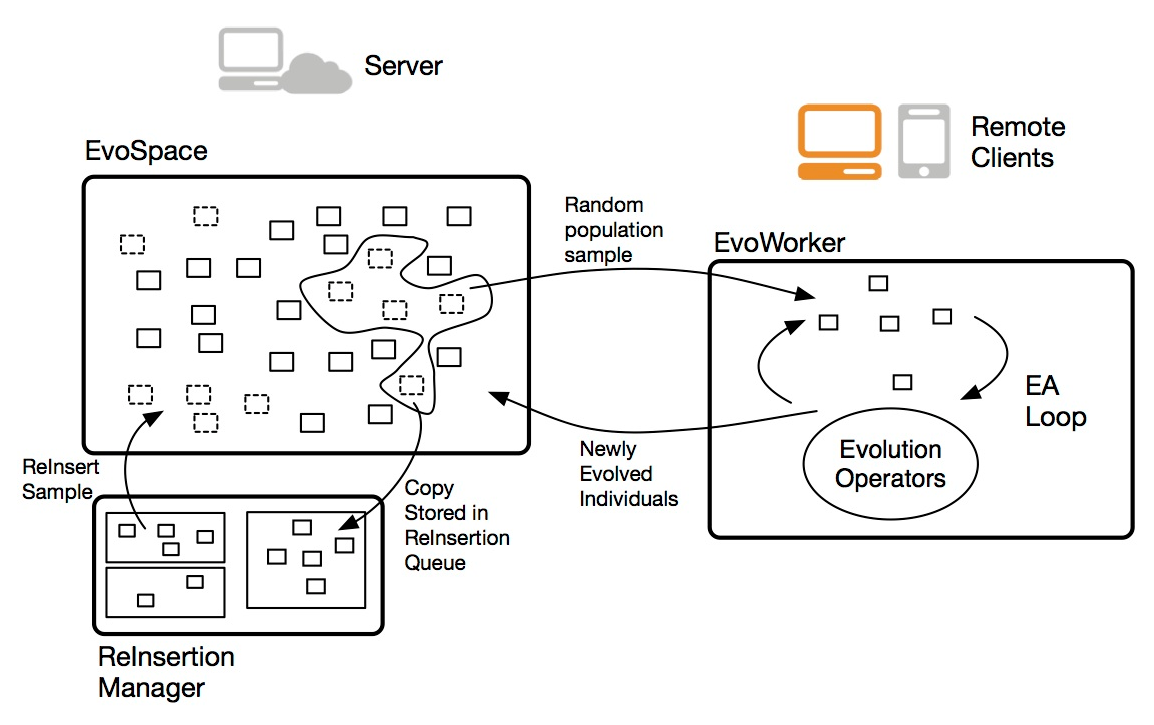
\includegraphics[width=4.5in]{eps/evospaceExample.eps}
    \caption{Main components and dataflow within EvoSpace.}
    \label{fig:evo}
\end{figure}


\subsection{Implementation}
Populations of individuals are stored in-memory, using Redis, a
key-value database, which 
 was chosen over a relational database system, or other non-SQL 
alternatives, because it provides a hash based implementation of sets 
and queues which are natural data structures for the EvoSpace model. 
The logic of EvoSpace is implemented as a python module and exposed as a web 
service using Cherrypy http library. The EvoSpace modules are available with 
a Simplified BSD License from 
% https://github.com/mariosky/EvoSpace. 
\url{anonymous URL}.

\subsection{Evospace as a Heroku Application}

Heroku (\url{http://heroku.com}) is a multi-language PaaS, supporting among others
Ruby, Python and Java applications. The basic unit of composition on
Heroku is a lightweight container running a single user-specified
process. These containers, which they call {\em dynos}, can include web
(only these can receive {\tt http} requests) and worker processes
(including systems used for database and queuing, for instance).
These  process types are the prototypes from which one or more dynos 
can be instantiated; if the number of requests to the server increases
more instances can be assigned on-the-fly. In our case, our CherryPy 
web application server runs in one web process, when the number 
of workers was increased we added more dynos (instances) of the 
CherryPy process.

This model is very different from a VPS where users pay for the
whole server; in a process based model, users pay only for the
processes they need; being a {\em freemium} model means also that, if
a minimum level of resources is not exceeded, it can be used for
free. 

Once deployed the web process can be scaled up by assigning more dynos;
in our case and in the more demanding configurations of our experiments, 
the web process was scaled to 20 dynos. Instructions and code for deployment 
is available at \url{anonymous URL} % Tienes
                                % que anonimizarlo tamibén - JJ
%http://www.evospace.org/software.html



\subsection{Evoworkers as PiCloud Jobs}
PiCloud is a Platform as a Service (PaaS), with deep Python integration; 
using a library, Python functions are transparently uploaded to PiCLoud's 
servers as units of computational work they call \emph{jobs}. 
Each job is added to a queue, and when there is a core available, 
the job is assigned to it. Both Heroku and PiCloud 
platforms are deployed  on top of Amazon Web Services (AWS) 
infrastructure in the US-EAST Region. This ensures minimal 
latency and a high bandwidth communication between the services, 
and there is no charge for data transfer costs between both services.
For the experiments type c1 and c2 Real Time workers where used.  
The code for the EvoWorkers implementation and experiment data is publicly available 
from a github repository \url{anonymous URL}. 
% \url{http://goo.gl/92tMFw}. % Github tiene su
                                % propio acortador, pero también
                                % tienes que anonimizarlo - JJ 

\section{Experimental work}
\label{sec:experiments}
\subsection{Benchmark}
\label{ss:benchmark}
The experiment reported here uses a multimodal problem generator. A P-Peaks generator
has been chosen because the problem (and the computing resources needed for the search) 
can be appropriately scaled. Proposed by De Jong et al. in \cite{Jong:PS97} a
P-Peaks instance is created by generating a set of P random N-bit
strings, which represent the location of the P peaks in the space. To
evaluate an arbitrary bit string \begin{math} \mathbf{x} \end{math}
first locate the nearest peak (in Hamming space). Then the fitness of
the bit string is the number of bits the string has in common with
that nearest peak, divided by N. The optimum fitness for an individual
is 1. This particular problem generator is a generalization of the
P-peak problems introduced in \cite{Jong:1990}.            

\begin{equation}
f_{P-PEAKS}(\mathbf{x})=\frac{1}{N} \overset{P}{\max_{i=1}} \{N-hamming(\mathbf{x},Peak_i)   \}
\end{equation}

A large number of peaks induce a time-consuming algorithm,
since evaluating every string is computationally hard; this is
convenient since to evaluate these type of distributed evolutionary
algorithms fitness computation has to be significant with respect to
network latency (otherwise, it would always be faster to have a
single-processor version). However
according to Kennedy and Spears \cite{Kennedy:1998ch} the length of
the string being optimized has a greater effect in determining how
easy or hard is the problem. In their experiments an instance having P
= 200 peaks and N = 100 bits per string is considered to produce a
considerably difficult problem.

\subsection{Experimental Set-up}
As EvoSpace is only the population store, EvoWorkers must implement 
the genetic operators. The genetic algorithm executed by EvoWorkers has been implemented 
using a modified DEAP (Distributed Evolutionary Algorithms in Python) 
framework \cite{DEAP_JMLR2012} GA. Is important to note that only the basic non-distributed GA 
library was used. Three methods were added to the local algorithm: 
{ \tt  getSample()} and  {\tt putBack()}; and  another for the  initialization 
of the population. The implementation of the local GA simply uses DEAP´s methods; for instance to 
generate the initial population, a local {\tt initialize()} is called 
and the population sent to EvoSpace.

The selection of parameters was based on those used in \cite{Alba:2002dq}: a
tournament size of 4 individuals, a crossover rate of 0.85 and a
population of 512 individuals. In  \cite{Jong:PS97} a mutation rate
equal to the reciprocal of the chromosome length; is recommended, as
DEAP uses two parameters they were defined as follows, mutation
probability of 0.5 and an independent flip probability of 0.02. For
EvoWorkers the parameters were 128 worker generations for each
sample, and a sample size of 16. To simulate unreliable workers each worker 
was assigned a return sample probability. In the experiments the lower 
probability was a 30\% chance of an EvoWorker returning a sample or
an EvoWorker failing 70\% of the time; other return sample probabilities
where 50\%, 70\% and 90\%. Experiments where carried out for 4, 
8 and 16 EvoWorkers. In a pool based  asynchronous GAs there is usually no need 
to wait for a worker´s job to start a new generation. Although supported by EvoSpace
time outs were not chosen as triggers to feed the population with new
individuals, the population size was used instead. We believe the population
size is a better threshold as it is more critical to the GA performance. 
In a previous work we found that when the population remaining in the pool 
was near starvation, the time of completion was increased. For these 
experiments, the insertion of individuals was triggered when less than 128
individuals remain in the population; the number of individuals feed to the
population was 128, or 8 samples when the re-insertion algorithm
was used. A summary of the setup is presented in table~\ref{params}.

\begin{table}[!t]
\renewcommand{\arraystretch}{1.3}
\caption{GA and EvoWorker parameters for experiments.}
\label{params}
\centering
\begin{tabular}{|l|c|}
\hline
\multicolumn{2}{|c|}{GA Parameters} \\
\hline
Tournament size & 4 \\
Crossover rate & 0.85  \\
Population Size & 512 \\
Mutation probability & 0.5 \\
Independent bit flip probability  & 0.02 \\
\hline
\multicolumn{2}{|c|}{EvoWorker Parameters} \\
\hline
Sample Size & 16 \\
Generations & 128 \\
\hline
\multicolumn{2}{|c|}{Other Parameters} \\
\hline
PiCloud Worker Type & Realtime \\
Number of Workers & 4,8,16 \\
Return Sample Probability & 30\%,50\%,90\% \\
Number of Executions & 30 \\

\hline

\end{tabular}
\end{table}

\begin{figure}[t]
\centering
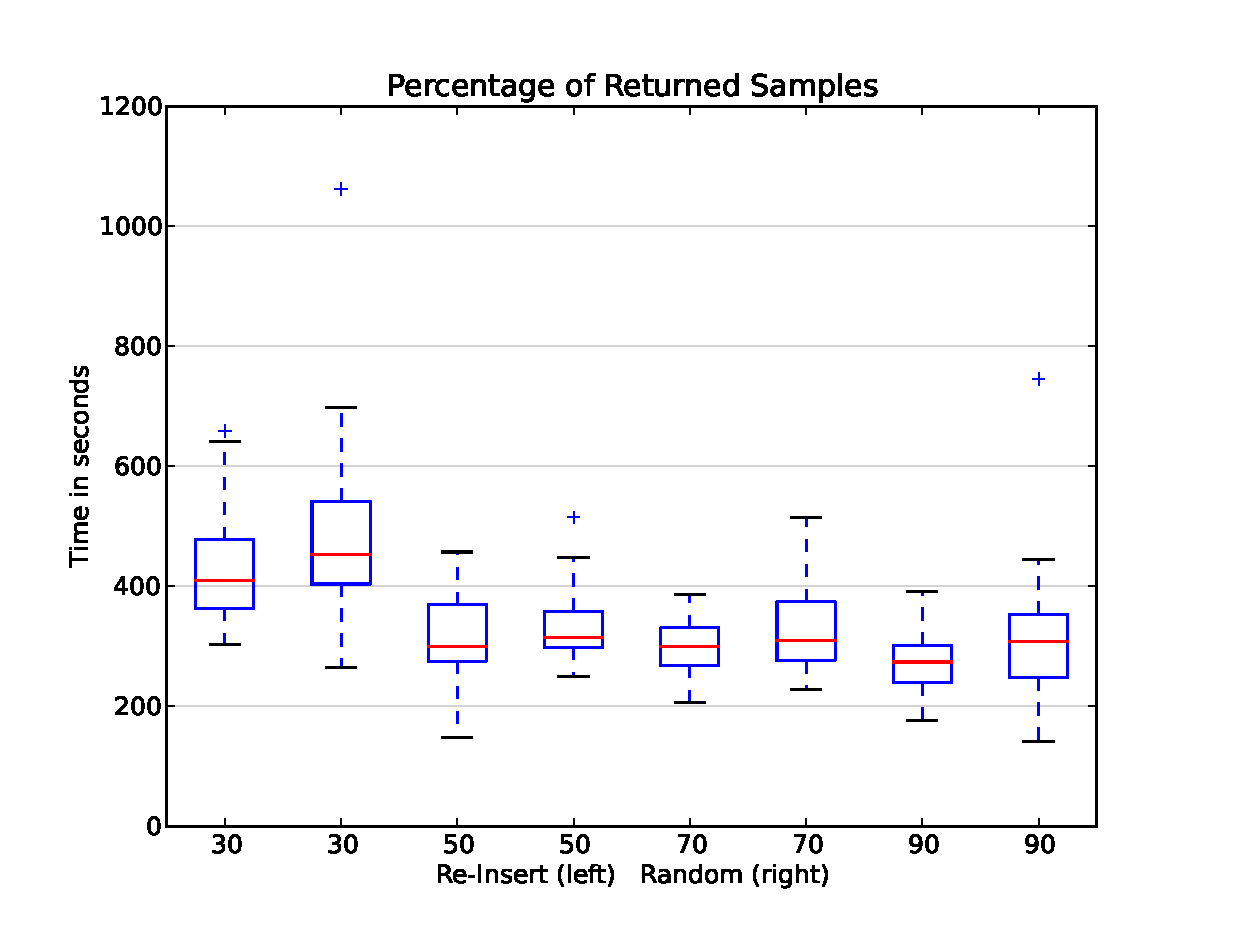
\includegraphics[width=3.5in]{eps/plot_time_CRS_w4.eps}
\caption{Time required to solution, 4 Workers}
\label{fig:plot_time_ri_w4}
\end{figure}

%Quizás deberías poner los random para el mismo número de
%eliminaciones al lado de reinsert, 30, 30, 50, 50 y así
%sucesivamente, sería más fácil compararlos. 
%% Hecho, Mario


\begin{figure}[!t]
\centering
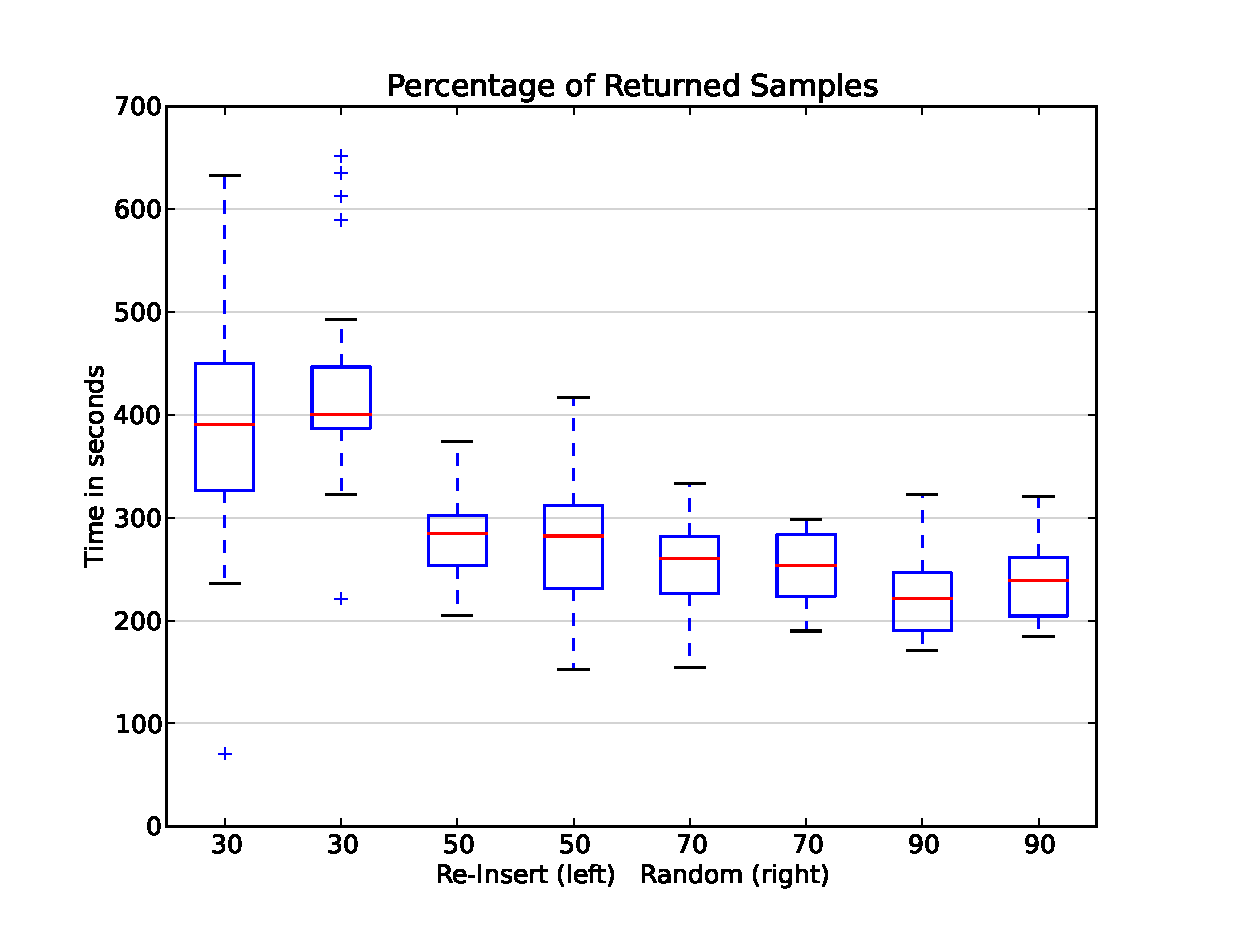
\includegraphics[width=3.5in]{eps/plot_time_CRS_w8.eps}
\caption{Time required to solution, 8 Workers}
\label{fig:plot_time_ri_w8}
\end{figure}


\begin{figure}[!t]
\centering
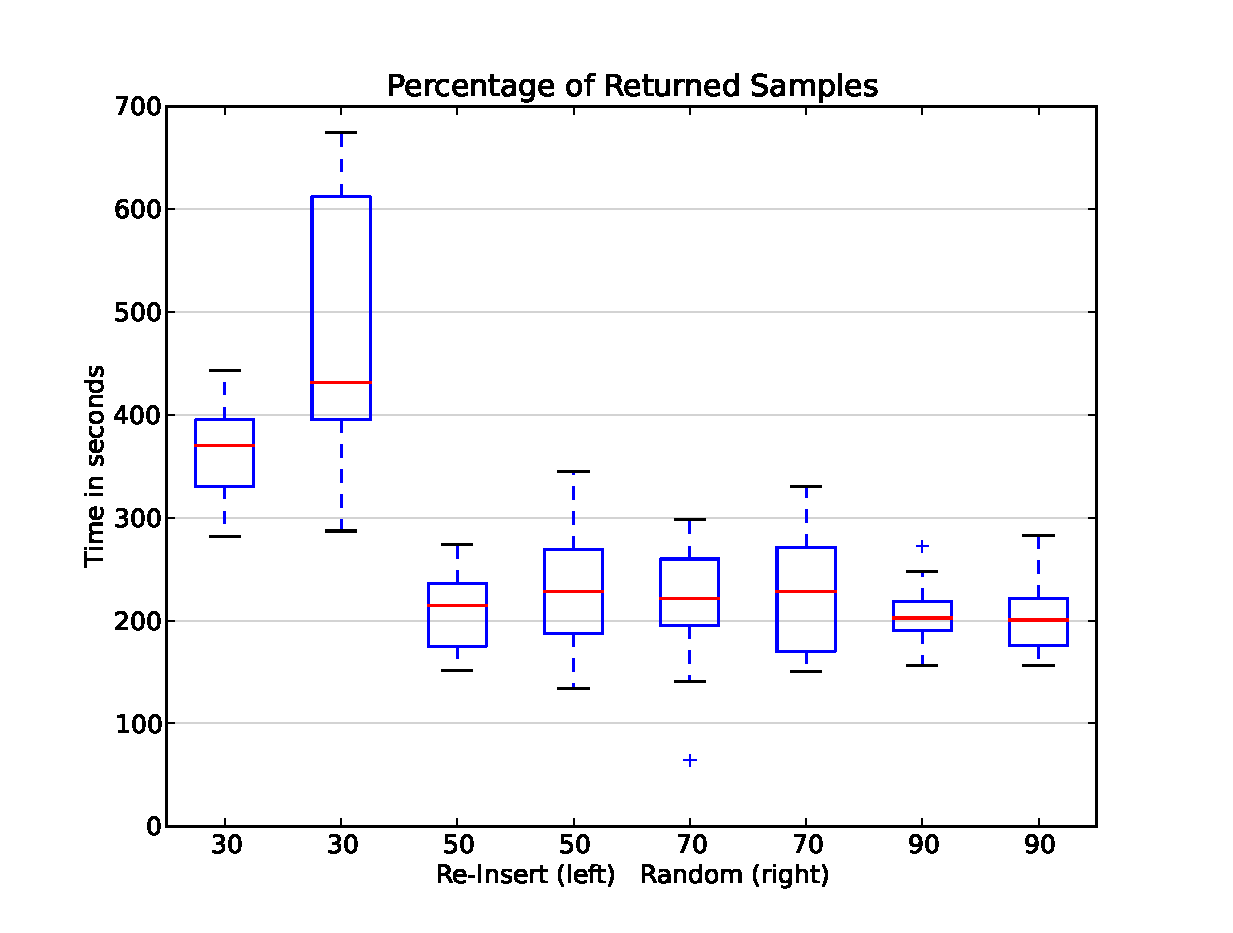
\includegraphics[width=3.5in]{eps/plot_time_CRS_w16.eps}
\caption{Time required to solution, 16 Workers}
\label{fig:plot_time_ri_w16}
\end{figure}


\begin{figure}[!t]
\centering
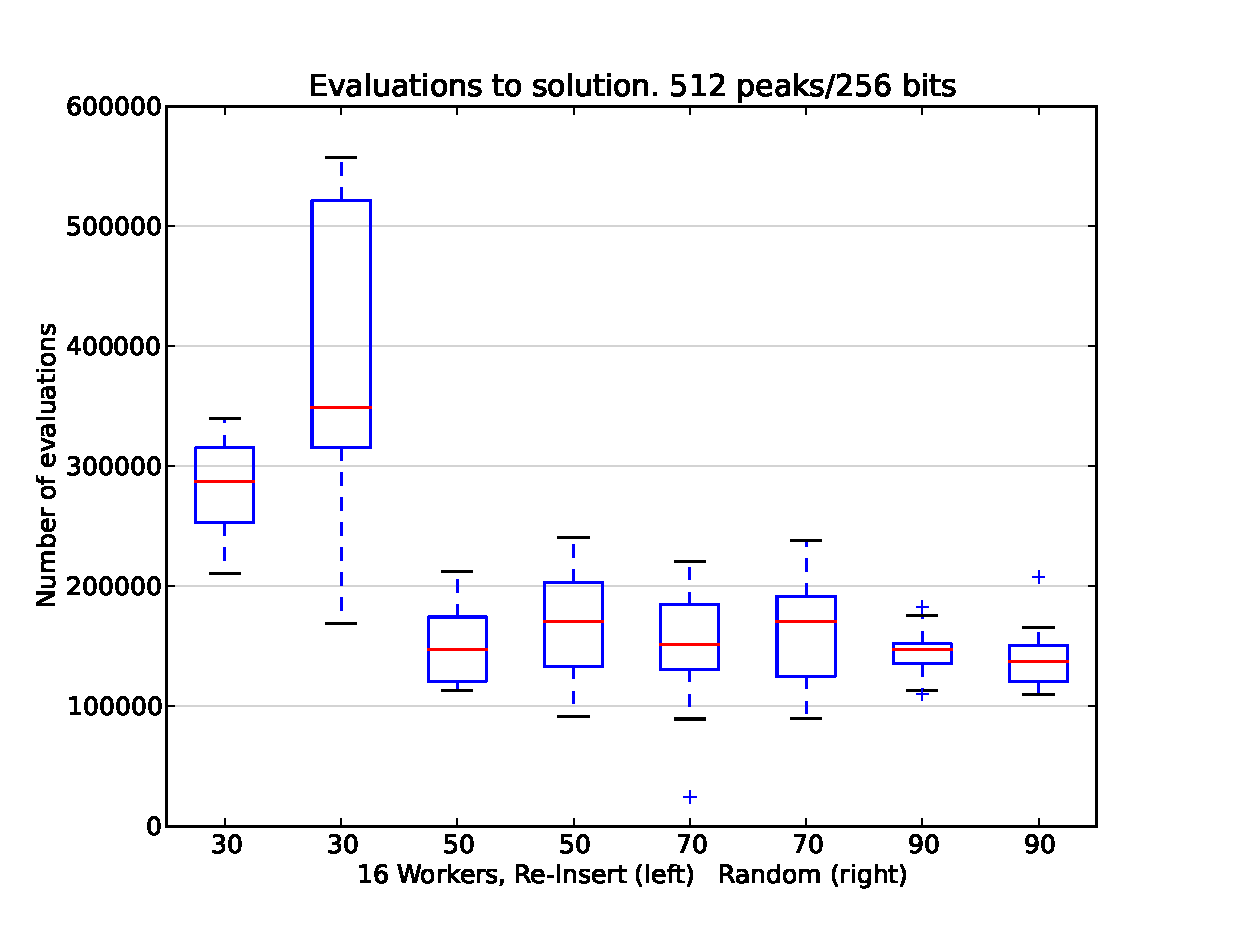
\includegraphics[width=3.5in]{eps/16_plot_evals.eps}
\caption{Number of evaluations needed to solution, 16 Workers}
\label{fig:plot_evals_w16}
\end{figure}

\begin{figure}[!t]
\centering
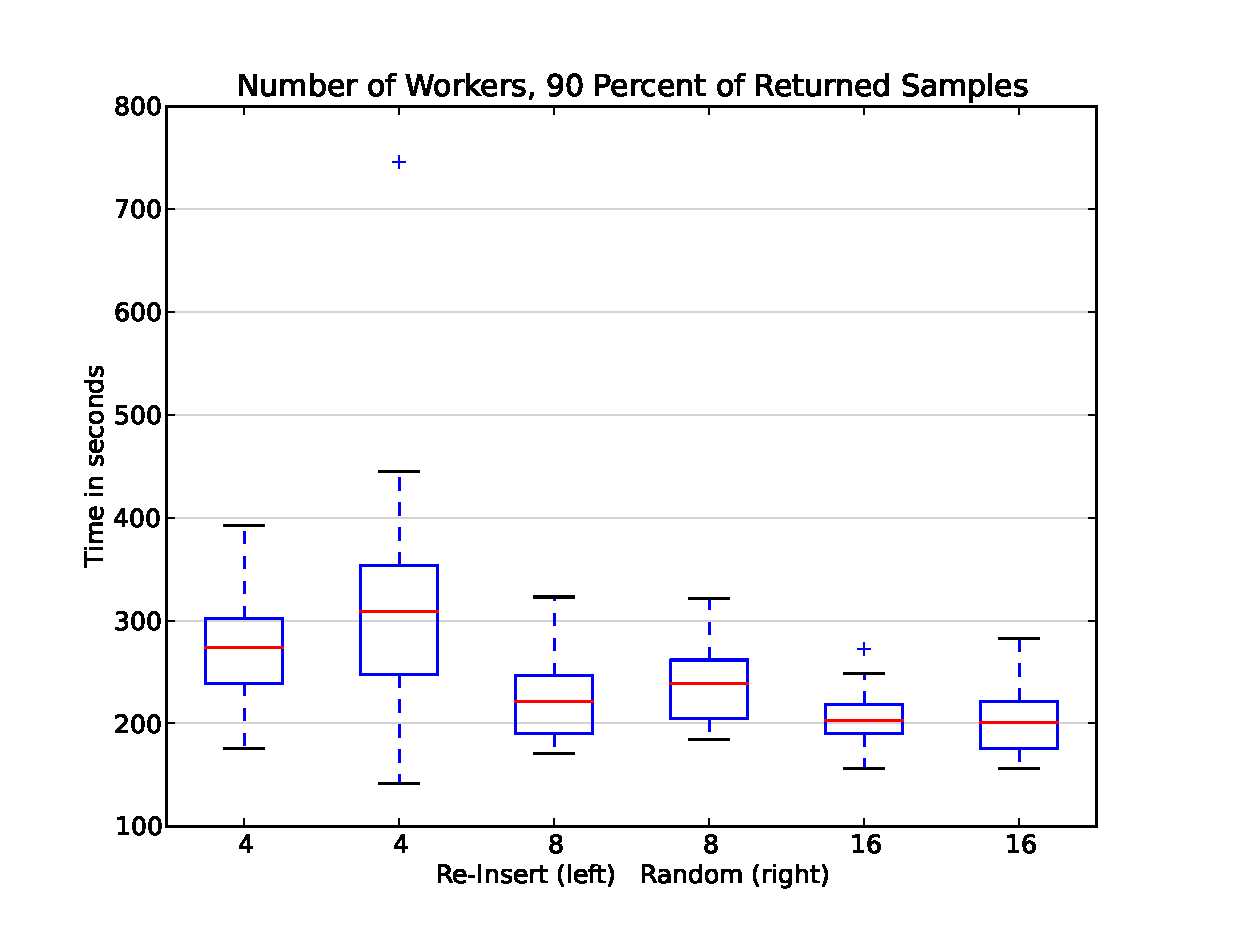
\includegraphics[width=3.5in]{eps/plot_percent_90.eps}
\caption{Time required to solution, 90\% of returned samples}
\label{fig:plot_percent_90}
\end{figure}

\begin{figure}[!t]
\centering
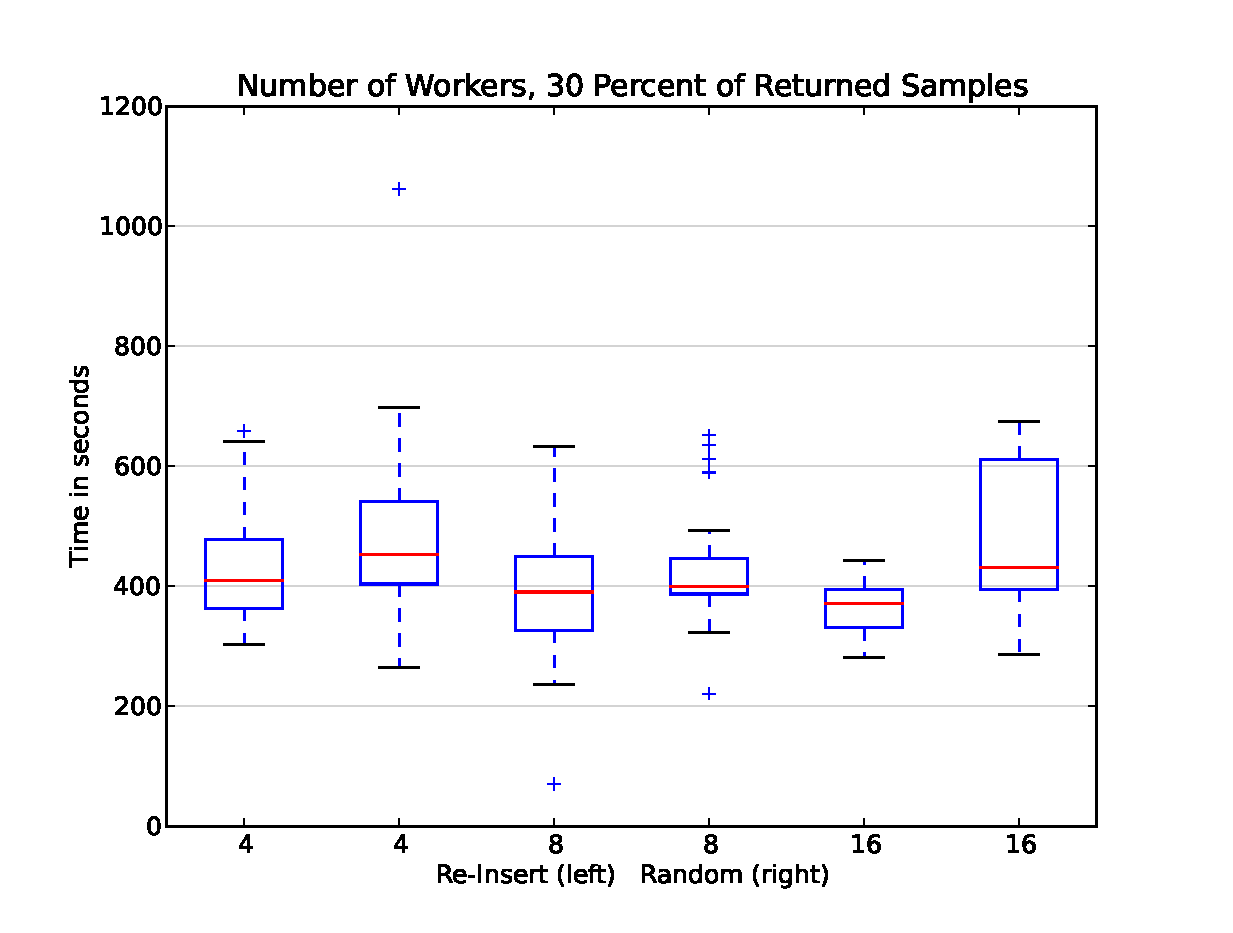
\includegraphics[width=3.5in]{eps/plot_percent_30.eps}
\caption{Time required to solution, 30\% of returned samples}
\label{fig:plot_percent_30}
\end{figure}

\begin{figure}[!t]
\centering
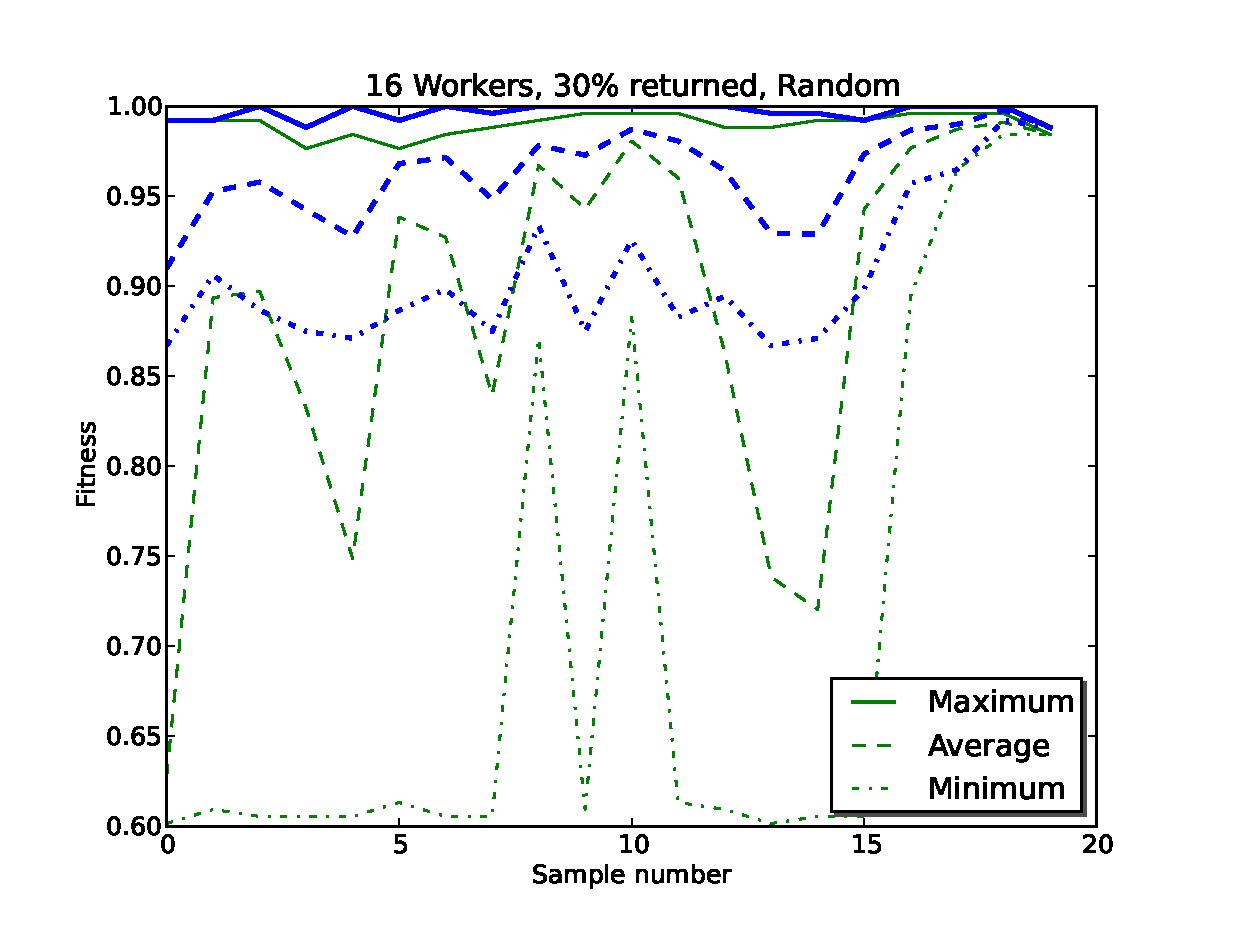
\includegraphics[width=3.5in]{eps/Fitness-w16-30-random.eps}
\caption{Fitness by Sample number, 30\% of returned samples, 16 Workers, Random Algorithm}
\label{fig:Fitness-w16-30-random}
\end{figure}

\begin{figure}[!t]
\centering
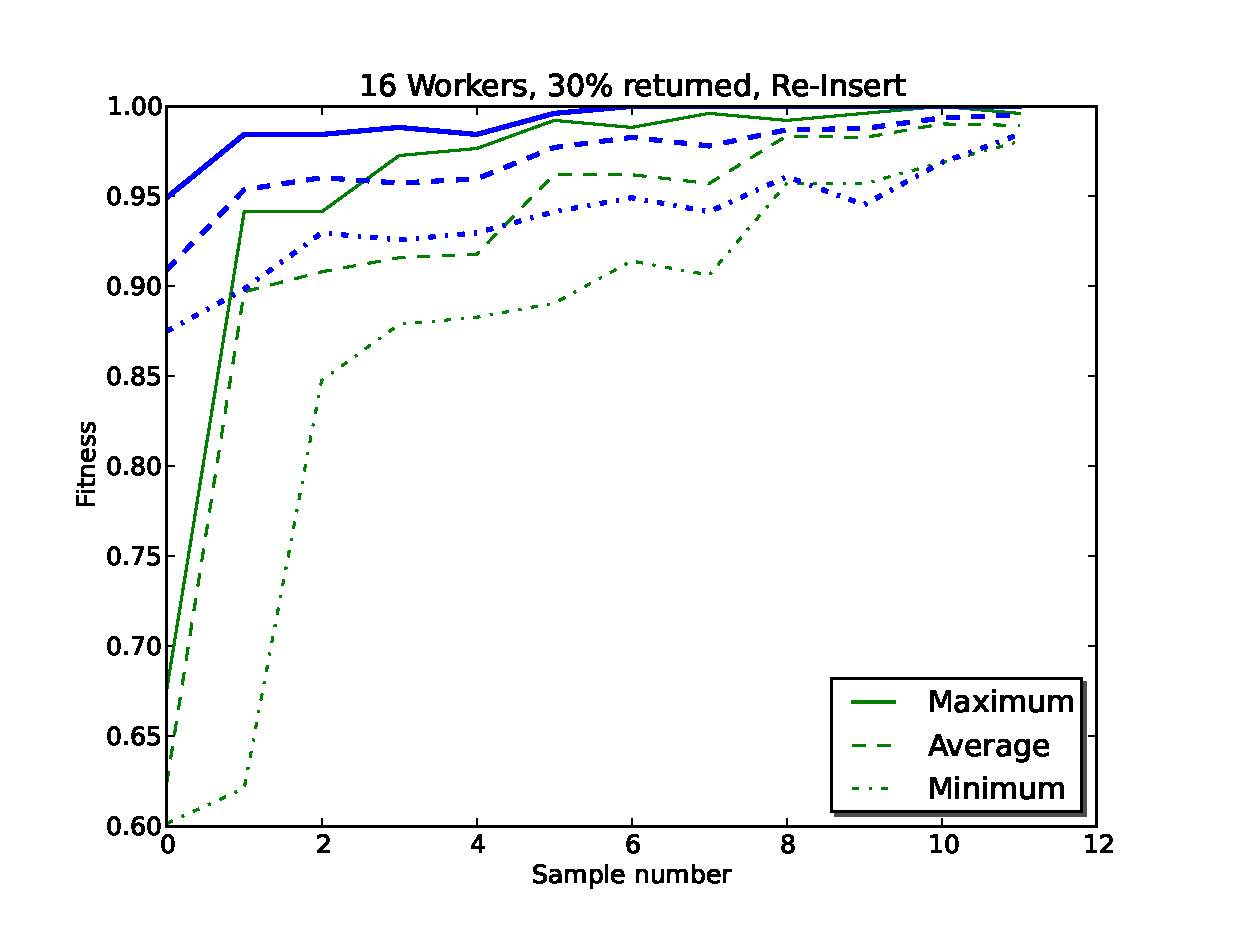
\includegraphics[width=3.5in]{eps/Fitness-w16-30-reinsert.eps}
\caption{Fitness by Sample number, 30\% of returned samples, 16 Workers, Re-Insert Algorithm}
\label{fig:Fitness-w16-30-reinsert}
\end{figure}


\subsection{Results}
In this section, results from the experiments are discussed. 
Figure~\ref{fig:plot_time_ri_w4} shows the time required 
to solution when using four EvoWorkers. For a population of
512 individuals and a sample size of 16, there is no
difference in the time required to solution for 
percentages of 50\% and above. Both re-insertion algorithms
had comparable times. For 30 percent, both approaches 
had slight increase in time. For 8 workers 
(see Figure~\ref{fig:plot_time_ri_w8})  there was marginal
decrease in overall time; and results where 
similar to those found in the experiments with 4 workers.  
Figure~\ref{fig:plot_time_ri_w16} shows results for 16 workers,
when there was only a 30\% chance of returning a sample 
the rate of re-insertions was high, approximately once every 35
samples. In this case, the insertion of random individuals 
resulted in a higher time to solution. For these experiments
when there is not a high rate of re-insertion, both alternatives
have similar results, but the re-insertion algorithm is better
for situations when there are many starvation conditions. It appears
that the insertion of random individuals is not detrimental when there
are other evolved individuals in the pool. But when the remaining
pool almost consists of random individuals, samples pulled by
EvoWorkers need to start the search all over again. 
If not many samples are then returned to the pool, the work needed to reach an
optimum is increased. Figure~\ref{fig:plot_evals_w16} also shows the number 
of evaluations needed to reach an optimum again for 16 workers.
Figures~\ref{fig:plot_percent_90} and \ref{fig:plot_percent_30} show
the time required to solution for 30 and 90 percent of returned samples.
For 90\% both algorithms had similar speedups when incrementing the number of
workers. The marginal speedup obtained for these experiments is related to 
the population size, but this parameter was not changed. For 30\% 
there was practically no speedup at all. The re-insert algorithm
although not significant, had consistent decrease in time.         

Fitness by time was measured as the average from each consecutive
sample pulled by each worker. For each sample the average fitness
was measured at the start and at the end of the local evolution.
Also the minimum and maximum fitness values at start and finish was 
recorded. Final fitness values are shown in double width lines in figures.
Readings used for these figures include all samples, including
those that where not returned.   
Figure~\ref{fig:Fitness-w16-30-random} shows fitness by time
for the random insertion algorithm, as expected initial fitness drops
at certain points, when random insertion occurs. Average final fitness 
is affected by random insertions.Figure~\ref{fig:Fitness-w16-30-reinsert}
shows results for the re-insertion algorithm, with more
characteristic curves for this type of algorithms. 
 
 

% Podrías comparar también el resultado para un porcentaje
% determinado, 90 y 30 para todos los números de workers y
% discutirlo. Es presentar los datos de otra forma solamente - JJ
%% Hecho, Mario

% Quizás también presentar como evoluciona el fitness en función del
% tiempo para los dos tipos de reinserciones y para el mínimo y máximo
% porcentaje de reinserción, para que se vea en qué fase del algoritmo
% influye más, principio o final o qué. Yo creo que al principio
% variará poco si es random o reinsertado - JJ 

% Habría que extender más esta sección de resultados y añadir algo de
% discusión. Al final queda un poco débil y va a ser difícil que lo
% admitan como trabajo, sólo como póster. - JJ

\section{Conclusions and Further Work}
\label{sec:conclusions}

The re-insertion algorithm proposed for EvoSpace is a viable alternative
to deal with a starving population in pool based GAs, and unreliable EvoWorkers.
Using  a benchmark problem from the P-Peaks problem generator, 
the approach was compared against the option of inserting  
randomly generated individuals. The same parameters and computing resources
were used when testing both algorithms with better times reported when
using the proposed technique. For experiments where the population
size is enough for the number of workers with their sample sizes, plus a 
buffer to account for loss samples, then both algorithms could be used.
However for cases when the number of EvoWorkers is unknown an hybrid approach
could be used, insertion of random individuals to gradually increase the population
size, and a re-insertion queue to handle lost samples. Further work could be
focused on a hybrid approach, and also using heterogeneous computing resources. 

\section{Acknowledgements}

Hidden for double-blind review. 

%
% ---- Bibliography ----
\bibliographystyle{abbrv}
\begin{footnotesize}
\bibliography{biblio}
\end{footnotesize}

\end{document}
